% Your original design document. Also, a discussion of what had to change over the course the year.

%%%%%%%%%%%%%%%%%%%%%%%%%%%%%%%%%%%%%%%%%%%%%%%%%%%%%%%%%%%%%%%%%%%%%%%%%%%%%%%%%%%%
\subsection{Introduction}
The Department of Integrative Biology at Oregon State has collected a large sample of biodiversity data from various sites in the United States.
Handling this data in its raw form requires certain technical knowledge of databases, as well as bit of patience.
This presents a problem for biodiversity researchers and Department of Defense land managers, who need to be able to understand and make decisions about this data easily.
Our team will address this problem by creating a web interface for spatially visualizing this data.
We will enable users to easily display useful statistics, graphs, and maps about areas and species of interest, putting the information they care about most at their fingertips.

The Department of Defense made an investment in collecting all these samples so that it could better manage its land.
However, extracting meaning from that information is challenging for land managers and researchers alike.
A good solution to this problem would allow users to easily access the information that is important to them.
Our solution will provide an interactive map overlaid with tools that allow users to easily select information of interest and display useful graphs and statistics about it.
Passerby at Expo will be invited to interact with our system and discover meaningful biodiversity information for themselves.
Oregon State biodiversity researchers and Department of Defense land managers will provide feedback on how well our product meets their needs.

\subsection{Project Plan}

\subsubsection{Requirements}
We will create a web interface for interacting with and visualizing the dataset provided to us.
This interface will be comprised of three main views: the map view, the statistics view, and the filter view.

The map view displays the region of interest on a map annotated with markers showing where data has been collected.
The user will be able to use this map to select the specific sites and areas they are interested in.
The sites that the user selects will be used to populate the charts and graphs so that they can see what is going on in that area.
This view will require the use of mapping software and a database in order to create the map itself and to populate it with markers corresponding to each site.

The statistics view takes the data from sites selected in the map view and renders statics, maps, and charts that make it easy to see trends and understand the data. Examples of these are: a graph of biodiversity over time, a Shannon diversity score, and a chart of the insect population by taxa or species.
This will be accompanied by any further kinds of statistics and comparisons that they feel would be useful for interpreting the data.
We will be creating these graphs and charts using NumPy/SciPy for doing the scientific calculations and using D3 to render the graphs and charts themselves.
The statistics view will also require that the data be in an accessible database form.

The filter view will display options that allow users to filter the data in the map and statistics views.
There will be several of these filters that can all be used together to give the user the exact data that they want.
The date filter allows users to specify what timeframe they are interested in.
The taxa filter will allow for viewing data related only to the selected taxa which includes species, order, genus, et cetera.
The site filter will allow users to select multiple sites with a unifying factor, such as all being in the same drainage basin.

\subsubsection{Timeline}

\begin{figure}[h]
	\centering
	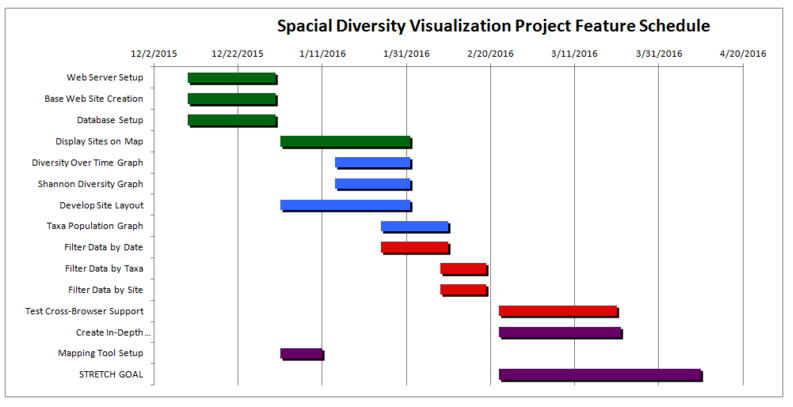
\includegraphics[width=0.95\textwidth]{OriginalGantt.png}
	\captionsetup{justification=centering}
	\caption{
		Gantt chart of schedule
	}
	\label{fig:original_gantt}
\end{figure}

The gantt chart above displays the plan for developing this website over the course of the next two terms.
We will start by setting up the foundation of the site by configuring the web server, importing the database, and deploying the basic framework.
The web server and dataset are provided by our sponsor. The dataset is not immediately in a mysql-import-ready state, but after some massaging we will import and set that up as well. 

After establishing the server, our plan is to add on functionality incrementally, increasing the functionality of the website.
Functionality will be added to the codebase in a modular fashion, each with their own branch in our version control system (git). 

Once our site is feature complete, we will begin our final steps for deployment.
We’ll have to test cross browser support to see how our site is handled by different clients.
We know we want to support browsers like edge, chrome, and firefox.
However, if we can manage supporting others that would be convenient.
After testing clients, we will polish our documentation and fill any gaps we missed along the way.
Documentation will be really important, both for usage and maintenance, because we will be handing this off to people who might not be familiar with our technology. 

Finally, our stretch goal will be to develop advanced statistical functions to run on the data.
This is something that has not been clarified yet and won’t be until the primary objective of the website is finished.
The general idea is to derive as much meaning from the data as possible, but in ways that still remain unknown.

\subsection{Design Plan}

\subsubsection{Database Specification}
The biodiversity data was initially recorded on paper, then was transcribed into a Microsoft Access database, and finally exported into an excel spreadsheet and given to us.
Needless to say, the data is a bit messy and not in an ideal form for use by our system.
We will be creating a database in the model described in the ER diagram in Figure ~\ref{fig:old_schema}.
We will need to create a script to map the raw data to our model.
The basic idea of the script will be to go through every line and extract all the information into their congruous constructs in the model.
This script will also involve some error checking as entering each entry completely by hand is a very error-prone process. 

\begin{figure}[h]
	\centering
	\includegraphics[width=0.95\textwidth]{old_schema.png}
	\captionsetup{justification=centering}
	\caption{
		ER diagram of database
	}
	\label{fig:old_schema}
\end{figure}

This model takes the simple records of the raw data and puts it in a relational database form.
This way information isn’t repeated and the records are usable by our systems.
In this model each species is broken off into its own table so it isn’t repeated for every single sample of that species.
This also has the benefit of making it easy to fix a mistake in spelling or change every instance of the species should the name change.
We do the same thing with the site, the data for the site is always the same so instead of attaching that data to every sample we simply put it in its own table for any sample in that area to reference.

Each trip to a site is modeled as a sample group that contains the the site that was visited, the date, and all of the various inorganic attributes that were recorded that day such as temperature, pH, and amount of silt in the water.
Each individual sample is a part of a group of sample and contains the number of instances that a given species was identified in the overall sample as well what percent it made of that sample.

\subsubsection{System Specification}
The back-end system will be written in a Python framework called Django. This back-end will handle how data is retrieved, manipulated, and sent to the rendered view in the user’s interface through a standard model-view-controller (MVC) practice. All of this processing will take place on the server side and will respond to requests from the client’s browser. The data flow diagram below outlines how the user will interact with the server to manipulate the data displayed.

\begin{figure}[h]
	\centering
	\includegraphics[width=0.95\textwidth]{DataFlowDiagram.png}
	\captionsetup{justification=centering}
	\caption{
		Gantt chart of schedule
	}
	\label{fig:data_flow}
\end{figure}

Upon first visit to the site the interface will fetch all records from the database to display by default. This means that all of the locations on the map where biodiversity data has been collected will be marked, initial statistics will be generated, and the filters will be empty. Once the main view has been rendered the user may begin to explore the map view or interact with the filter options.

Interacting with the filter options should immediately affect rendered data on the page. This means that after a checkbox has been checked/unchecked or a date range has been entered the data should reflect this change. As shown in the data flow diagram above, the user’s filtration params will be handled by an asynchronous function that will send a request to the server outside of the site’s main thread. It is important that this handler is asynchronous, because it means the page will not refresh and upon the return of a filtered dataset from the database the rendered content will be newly generated (i.e., the map shows only those qualifying locations as marked, the statistics are generated from that dataset, etc.).

Controllers:
The controller's purpose is to receive specific requests for the application. Routing decides which controller receives which requests. Often, there is more than one route to each controller, and different routes can be served by different actions. Each action's purpose is to collect information to provide it to a view. Whether there will be one primary controller for the site’s interface or 3 discrete controllers for each view within the interface is still up to which will be more convenient, since we haven’t gotten to the implementation phase yet. 

Views:
A view's purpose is to display this information in a human readable format. The view should just display that information. Our views will be three discrete files that are compiled into one main view for the user using a templating system. The details of how the views will work are part of the interface specification in the next section. 

Models:
The model is meant to map the objects in the database to code objects manipulatable by 
the controllers. Each model will have private functions that allow us to access attributes and perform logic depending on the situation. 

\subsubsection{User Interface Specification}

The user interface will consist of three views: the Map View, the Filter View, and the Statistics View. These will be tiled on the page as shown below. There will be one full length tile on the left, and two half-length tiles on the right. By default, the Map View will be in the left tile, the Filter View will be in the top right tile, and the Statistics View will be in the bottom right tile. Each view will have a bar at the top of its tile that identifies the name of the view. Each bar will have its own color.

\begin{figure}[h]
	\centering
	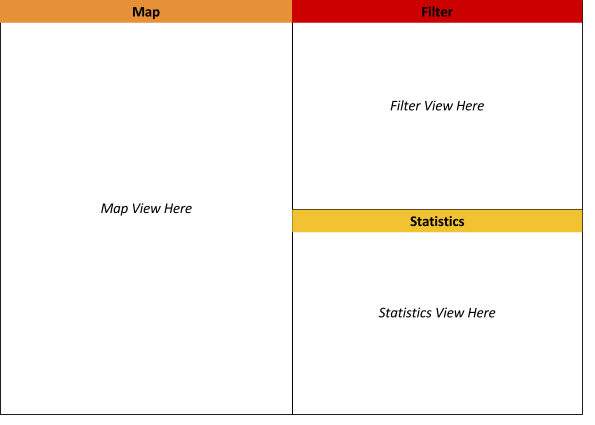
\includegraphics[width=0.95\textwidth]{Overview.png}
	\captionsetup{justification=centering}
	\caption{
		User Interface Mockup
	}
	\label{fig:overview}
\end{figure}


\subsubsection{Map View Specification}
The Map View will render a map of the area being studied using ArcGis that will be annotated with markers for each site that samples have been collected at. Users will be able to select sites by clicking on them individual or by dragging a box over the area they are interested in. Once they have selected their sites, the Statistic View will render the current graphs and charts with the new set of data.

Which sites are rendered is dependent on the settings in the Filter View, for instance, if you select a general area only sites in that area will be displayed and if you select a date range only sites that have data for that date range will be displayed. Figure 5 below shows a basic idea of what the map part of the Map View will look like.

\begin{figure}[h]
	\centering
	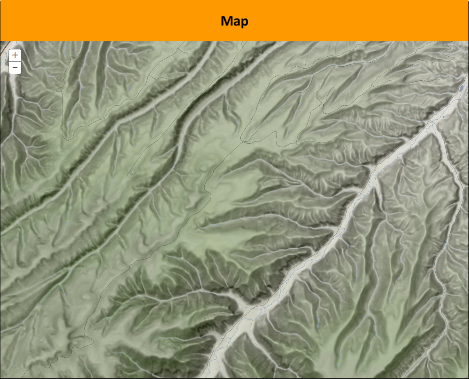
\includegraphics[width=0.95\textwidth]{map_mockup.png}
	\captionsetup{justification=centering}
	\caption{
		Map Mockup using ArcGis
	}
	\label{fig:map_mockup}
\end{figure}

Our Map View will look very similar Figure~\ref{fig:map_mockup}, but with colored markers showing the sites. These markers will need to update to show when they’ve been selected which we will do by changing the color of selected markers. Almost all of the functionality we need in the Map View will come from the ArcGis API, the markers, the geographical map, and the basic map manipulation features such as zooming and panning.

\subsubsection{Statistics View Specification}
The Statistics View will be generated using the C3.js libraries after being supplied data from our system’s controllers. This library was chosen because it has great responsive capabilities, an easy to customize api, and a wide variety of graphs and charts to choose from. As you can see in the mockup below there is a on-hover element in each graph for when a user’s cursor hovers or clicks a graph point. It will show the exact values for that data point, which is convenient for getting a quick and exact measure. The user can also hide / display data sets by simply clicking their name in the legend for dynamic visualization. The C3.js api allows for complete aesthetic control over the charts along with graphing options for different types of charts. 

The statistics view will either scroll upwards or sideways to allow for several meaningful interpretations of the data that we can display. As the user interacts with the filter view the data supplied to the graphs and charts will be re-generated to match the resulting dataset. The exact type of graphs and statistics to be displayed in this view are still being decided by David Lytle and his lab so that will be subject to much change throughout development. 

\begin{figure}[h]
	\centering
	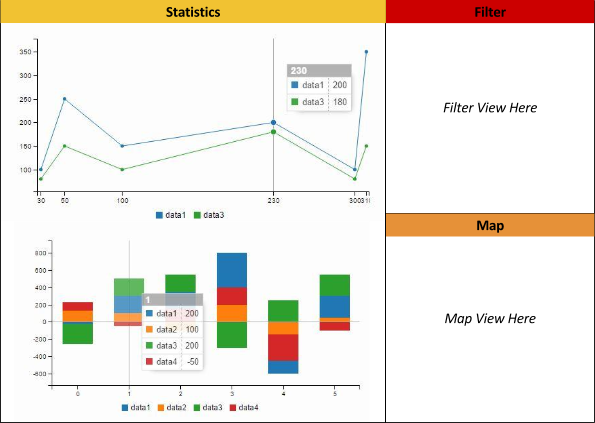
\includegraphics[width=0.95\textwidth]{statistics_mockup.png}
	\captionsetup{justification=centering}
	\caption{
		Statistics Mockup
	}
	\label{fig:statistics_mockup}
\end{figure}

\subsubsection{Filter View Specification}
The Filter View will allow the user to select information of interest with three filters: the Species Filter, the Site Filter, and the Date Filter.

The Species Filter will allow the user to select biological taxa hierarchically. Each line in the Species Filter will consist of a checkbox, a drilldown, and a name. At the top level will be the phylum Arthropoda. By default, this will be checked and the drilldown will be collapsed, as shown below.

The Site Filter will allow the user to select watersheds hierarchically. Each line in the Site Filter will consist of a checkbox, a drilldown, and a name. At the top level will be the various basins to which sites belong. By default, all basins will be checked and the drilldowns collapsed, as shown below.

The Date Filter will allow the user to select information by date. It will consist of a start date field and an end date field. By default, these will be set to the first and last samples recorded, respectively.

\begin{figure}[h]
	\centering
	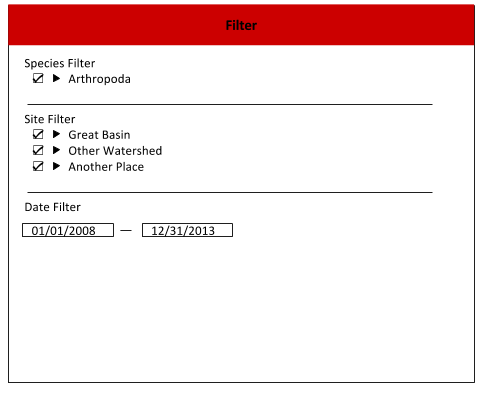
\includegraphics[width=0.95\textwidth]{filter.png}
	\captionsetup{justification=centering}
	\caption{
		Filter View Collapsed
	}
	\label{fig:filter_mockup}
\end{figure}

In the Species and Site Filters, clicking on a collapsed drilldown will expand it. This means that underneath that entry, the first level children will appear indented. Clicking on an expanded drilldown will collapse it. Bottom-level children will have no drilldown.

For the Species Filter, the top level will be the phylum Arthropoda. The next level will consist of all the classes of arthropods that appear at least once in the data. The next level will be all the orders that appear at least once in each of the classes, and so on down to the species.

For the Site Filter, the top level will be all the basins represented in the data. The second level will be all the sites at which samples were taken. The Site Filter will only have these two levels.

In the Species and Site Filters, checkboxes will have three states: checked, unchecked, and partially checked. If a taxon is checked, then all of its children are checked. If it is unchecked, then all of its children are unchecked. If it is partially checked, then some of its children are checked and some are unchecked. Clicking on a checkbox will recursively invert its selection. That is, clicking on a checked checkbox will uncheck it, all of its children, all of its children’s children, and so on. Clicking on an unchecked checkbox will check it, its children, its children’s children, and so on. Clicking on a partially selected checkbox will check all of its unchecked children and uncheck all of its checked children, and do the same for its children’s children, and so on.

As an example, the user below clicked on the drilldowns for Arthropoda, Insecta, Hemiptera, Hymentoptera, Apidae, Apis, and Orthoptera in the Species filter and for Another Place in the Site Filter. She then clicked on the checkbox for Orthoptera, unchecked all its children. She then unchecked some of Hemiptera’s children, then collapsed its drilldown. She also changed the dates in each field of the Date Filter.

\begin{figure}[h]
	\centering
	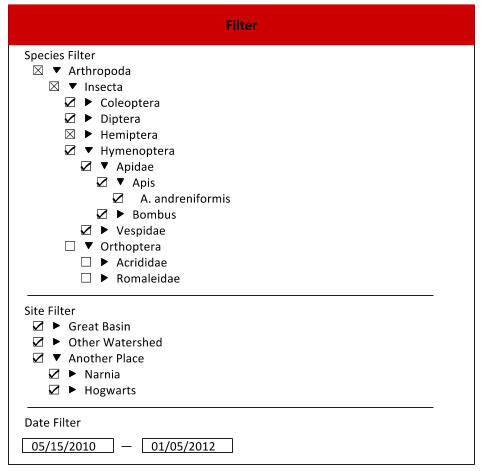
\includegraphics[width=0.95\textwidth]{filterinuse.png}
	\captionsetup{justification=centering}
	\caption{
		Filter view expanded
	}
	\label{fig:filter_mockup_in_use}
\end{figure}

\subsection{Changes}


